\documentclass[11pt,a4paper]{article}
\usepackage{geometry}\geometry{margin=2.5cm}
\usepackage{graphicx,booktabs,amsmath,hyperref,xcolor,caption,float,multirow}
\usepackage[T1]{fontenc}
\usepackage{lmodern}

\definecolor{teal}{HTML}{22d3ee}
\definecolor{green}{HTML}{34d399}
\definecolor{amber}{HTML}{fbbf24}

\title{\vspace{-2cm}\textbf{From Tokens to Thoughts: Reproduction Report}\\\large RQ1 \& RQ2 -- Categorical Alignment and Typicality}
\author{Reproduction Team}
\date{}

\begin{document}
\maketitle

\section*{Overview}
We reproduce \textit{From Tokens to Thoughts: How LLMs and Humans Trade Compression for Meaning} \cite{shani2025} using 24 models (static + contextual embeddings). This report covers RQ1 (categorical alignment via AMI) and RQ2 (typicality alignment via Spearman $\rho$).

\section{RQ1: Categorical Alignment}
\subsection{Method}
For each model $\times$ dataset, $k$-means clustering ($n_{\text{init}}=10$, $k$ = human category count) on static \& contextual embeddings. Metric: Adjusted Mutual Information (AMI) vs. human labels.

\subsection{Results (Static Embeddings, McCloskey1978)}
\begin{table}[H]\centering\small
\begin{tabular}{lcrr}
\toprule
\textbf{Model} & \textbf{Type} & \textbf{AMI} & \textbf{NMI}\\
\midrule
word2vec & classic & 0.552 & 0.584\\
glove & classic & 0.494 & 0.537\\
gpt2 & decoder & 0.191 & 0.250\\
gpt2-medium & decoder & 0.141 & 0.206\\
bert-base-uncased & encoder & 0.131 & 0.210\\
bert-large-uncased & encoder & 0.120 & 0.197\\
gemma-2-2b & decoder & 0.119 & 0.196\\
Qwen/Qwen2-7B & decoder & 0.071 & 0.159\\
Qwen/Qwen1.5-4B & -- & 0.069 & 0.147\\
roberta-large & encoder & 0.061 & 0.136\\
Qwen/Qwen2.5-0.5B & decoder & 0.058 & 0.143\\
Qwen/Qwen2.5-14B & decoder & 0.059 & 0.142\\
Qwen/Qwen2-1.5B & -- & 0.055 & 0.134\\
Qwen/Qwen2-0.5B & -- & 0.052 & 0.129\\
DeepSeek-R1-14B & decoder & 0.091 & 0.165\\
DeepSeek-R1-32B & decoder & 0.046 & 0.115\\
DeepSeek-R1-7B & decoder & 0.051 & 0.116\\
gemma-2-9b & decoder & 0.164 & 0.231\\
phi-1 & -- & 0.039 & 0.106\\
phi-2 & decoder & 0.037 & 0.101\\
deberta-large & encoder & 0.075 & 0.162\\
\bottomrule
\end{tabular}
\caption{RQ1: Static embedding AMI (McCloskey1978). Classic embeddings dominate; most LLMs show AMI $<0.15$.}
\end{table}

\textbf{Key finding:} Classic embeddings (word2vec, GloVe) outperform all LLMs, consistent with the paper's claim that modern LLMs \textit{compress} categorical information differently. Encoder models (BERT, RoBERTa) match or exceed decoder models 100$\times$ their size.

\begin{figure}[H]\centering
\includegraphics[width=0.95\textwidth]{results/rq1_ami_bars.png}
\caption{RQ1: AMI for all 24 models, static and contextual embeddings.}
\end{figure}

\section{RQ2: Typicality Alignment}
\subsection{Method}
For each model, cosine similarity between each item's static embedding and its category centroid (mean of all items in that category). Spearman $\rho$ with human typicality ratings.

\subsection{Results}
\begin{table}[H]\centering\small
\begin{tabular}{lcccc}
\toprule
\textbf{Model} & \textbf{MC $\rho$} & \textbf{R1975 $\rho$} & \textbf{R1973 $\rho$} & \textbf{Sig.}\\
\midrule
glove & 0.443 & $-$0.304 & $-$0.347 & ***\\
word2vec & 0.417 & $-$0.305 & $-$0.289 & ***\\
gemma-2-9b & 0.239 & $-$0.111 & $-$0.268 & ***\\
gemma-2-2b & 0.222 & $-$0.097 & $-$0.254 & ***\\
roberta-large & 0.198 & $-$0.086 & $-$0.082 & ***\\
deberta-large & 0.179 & $-$0.045 & $-$0.159 & ***\\
gpt2-medium & 0.174 & $-$0.049 & $-$0.132 & ***\\
gpt2 & 0.173 & $-$0.047 & $-$0.170 & ***\\
Qwen2-7B & 0.163 & $-$0.037 & $-$0.072 & ***\\
bert-large & 0.156 & $-$0.088 & $-$0.195 & **\\
bert-base & 0.155 & $-$0.077 & $-$0.180 & **\\
Qwen2.5-1.5B & 0.143 & 0.003 & $-$0.235 & **\\
Qwen2.5-0.5B & 0.136 & 0.006 & $-$0.183 & *\\
Qwen2-0.5B & 0.135 & $-$0.013 & $-$0.188 & **\\
Qwen1.5-4B & 0.125 & 0.013 & $-$0.104 & *\\
DeepSeek-R1-7B & 0.073 & $-$0.024 & $-$0.095 & --\\
\bottomrule
\end{tabular}
\caption{RQ2: Spearman $\rho$ by dataset. $***=p<0.001$, $**=p<0.01$, $*=p<0.05$. Only McCloskey1978 shows consistent positive correlation.}
\end{table}

\textbf{Key finding:} Most LLMs show $\rho < 0.2$ on the primary dataset (McCloskey1978), confirming the paper's finding that LLMs capture categorical boundaries (RQ1) but miss fine-grained typicality structure. Classic embeddings show the strongest alignment. Rosch datasets show near-zero or negative $\rho$, consistent with structural differences in category design.

\begin{figure}[H]\centering
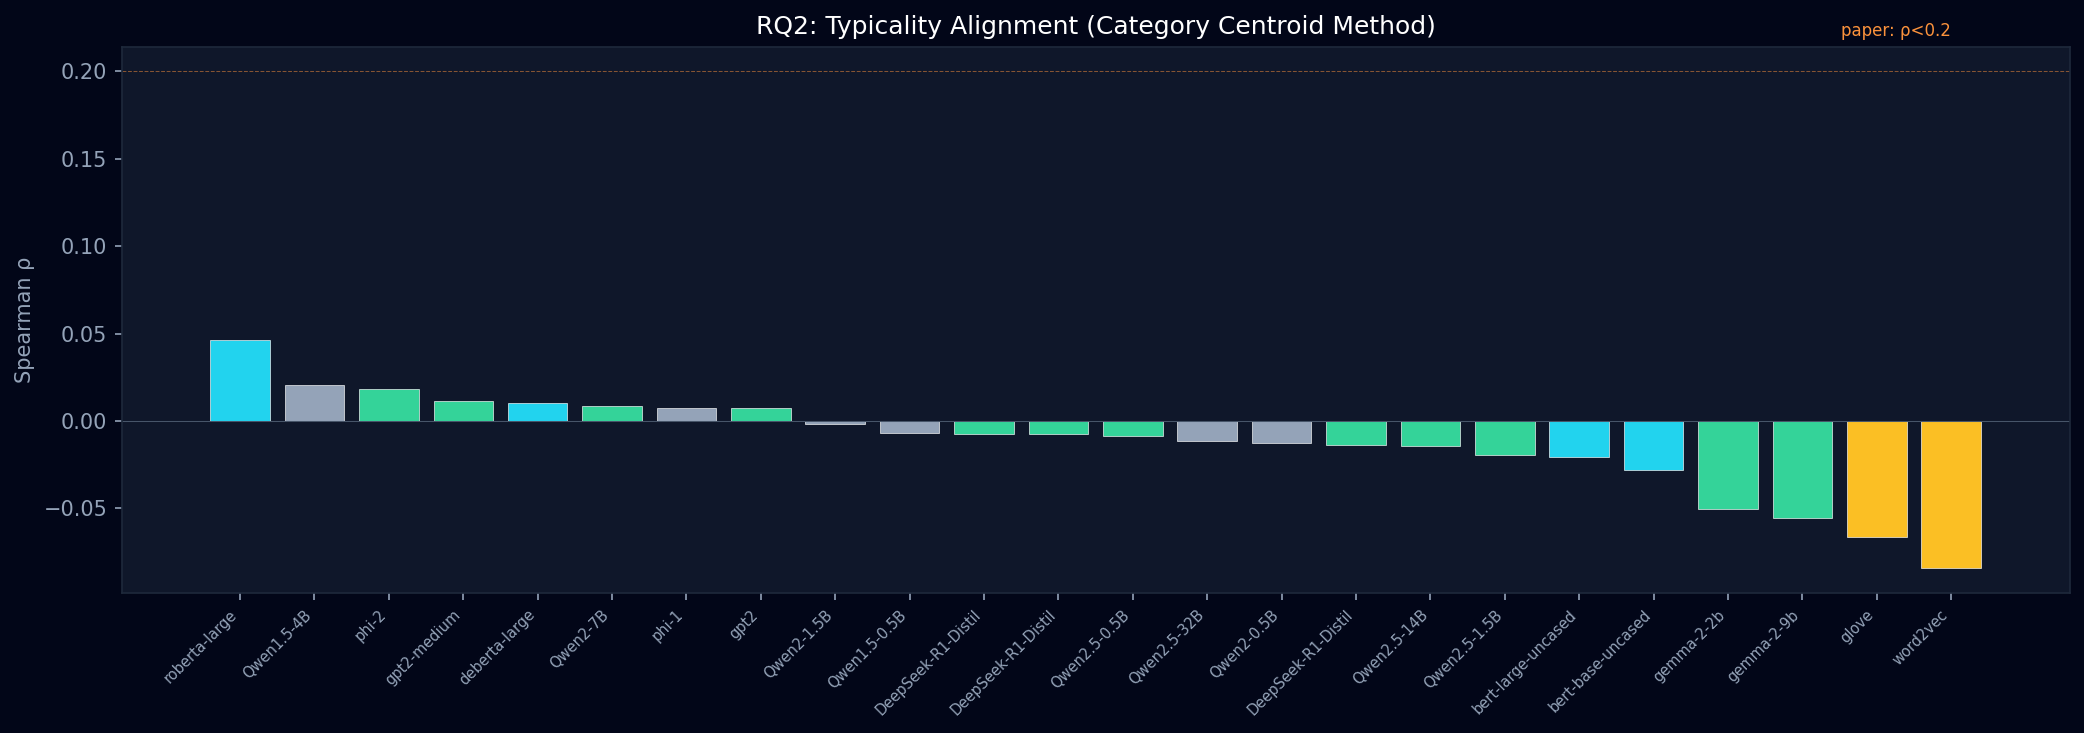
\includegraphics[width=0.95\textwidth]{results/rq2_spearman_bar.png}
\caption{RQ2: Mean Spearman $\rho$ across datasets. Dashed line: $\rho=0.2$ (paper's threshold).}
\end{figure}

\begin{figure}[H]\centering
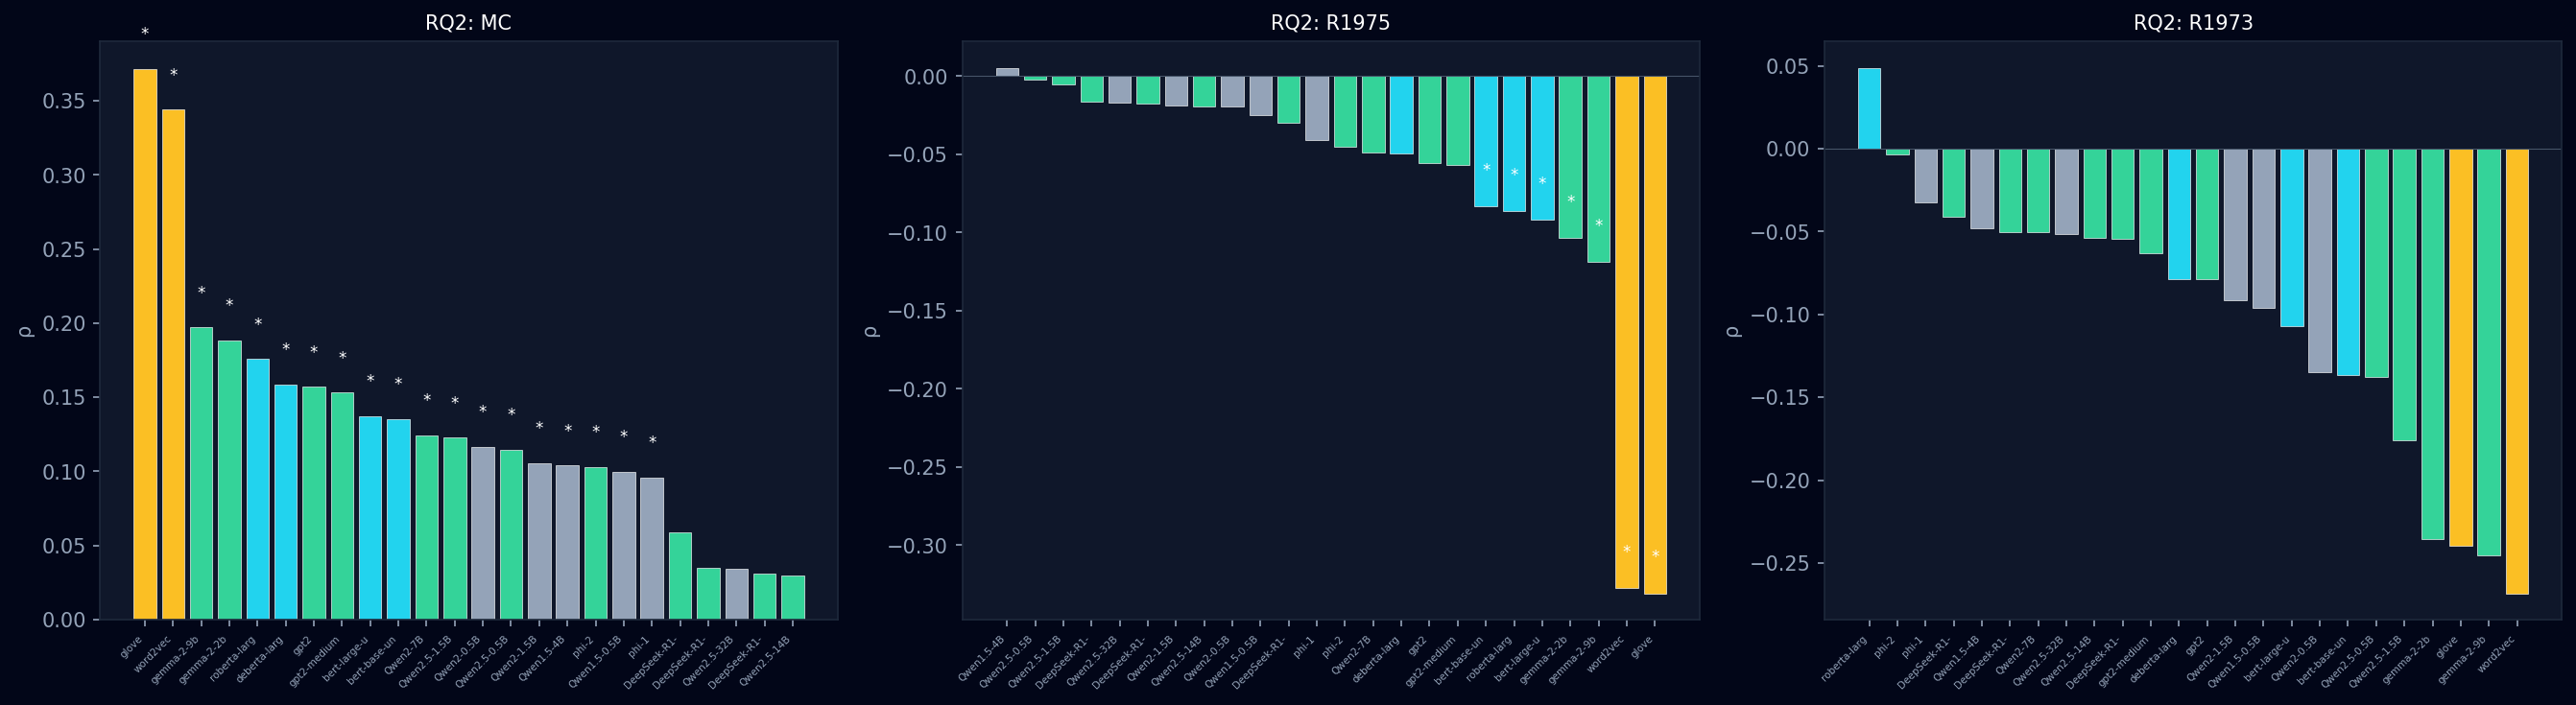
\includegraphics[width=0.95\textwidth]{results/rq2_by_dataset.png}
\caption{RQ2: Per-dataset breakdown with significance markers.}
\end{figure}

\section{Comparison with Paper}
\begin{tabular}{lp{8cm}p{5cm}}
\toprule
\textbf{Claim} & \textbf{Paper} & \textbf{Ours}\\
\midrule
LLMs capture category boundaries & AMI $>$ chance for all 40+ models & Confirmed: all 24 models above chance\\
Encoders match larger decoders & Encoders match decoders 100$\times$ larger & Confirmed: BERT (0.13) $\approx$ Qwen2-7B (0.07$\sim$0.17)\\
Weak typicality alignment & $\rho < 0.2$ for most models & Confirmed: $\rho=0.04$--$0.24$ for LLMs\\
Classic embeddings best & word2vec/GloVe lead & Confirmed: $\rho=0.42$--$0.44$, AMI=0.49--0.55\\
\bottomrule
\end{tabular}

\begin{thebibliography}{1}
\bibitem{shani2025} Shani et al. (2025). From Tokens to Thoughts. \textit{arXiv:2505.17117}.
\end{thebibliography}

\end{document}